\section{Zhodnocení}
Boid je velmi nenáročný na výpočetní výkon. Je možné jej paralelizovat, případně počítat na grafické kartě. 
\par
Výhoda modelu Boid spočívá v absenci detekce kolizí. Pokud mají agenti nastavenou správnou váhu, udržují si od sebe navzájem dostatečně velkou vzdálenost a není potřeba kolize počítat. 

\subsection{Problémy}
Přestože jednotliví agenti vykazují známky složitého chování, stále se řídí jednoduhými pravidly, které mohou zapříčinit nechtěné odchylky. Jednou z nich je tzv. semknutí dvou agentů, kteří se navzájem přetlačují a jeden druhému nedokáží ustoupit. To má za následek nechtěnné chování, kdy tito agenti většinou opustí hejno a může zapříčinit, že začnou procházet překážkami. 
\begin{figure}[H]
	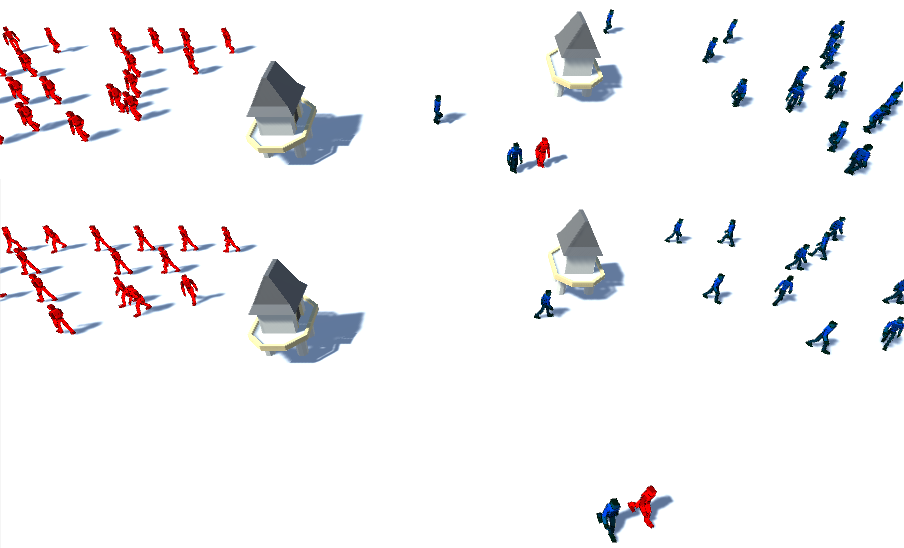
\includegraphics[width=10cm]{people_problem_anim.png}
	\centering
	\caption{Srážka a semknutí dvou agentů v časech $t\in\{ 100, 115\} $}
\end{figure}
Jednotlivá pravidla modelu jsou nastavena tak, aby se model pokusil vyhýbat kolizím, ale nedokážou zajistit 100\% úspěšnost. Do jisté míry se tento problém dá oddálit správným nastavením vah. První testy chování Boid modelu dosahovaly přibližně 200 kolizí\\s. Postupně se podařilo chování vyladit až na verzi bez žádné kolize. 
\par
Rozšíření o pravidlo vyhýbaní se překážkám, které Reynolds popsal ve své práci \cite{ReynoldsBoidNoBump} pracuje pouze se statickými objekty. Abhinav Golas, Rahul Narain a Ming Lin publikovali v roce 2014 článek Hybrid Long-Range Collision Avoidance for Crowd Simulation \cite{Golas2013}. Ve své práci popisují agenta, který umí predikovat pohyb jiných agentů a vyhnout se tak kolizi daleko dříve. 